\documentclass{beamer}
\usepackage{fontspec}
\usepackage{bm}
%\usepackage{unicode-math}
\usepackage{xcolor}
\usepackage{setspace}
\usepackage{microtype}

\usefonttheme{professionalfonts}
%\setmathfont{Latin Modern Math}

\setsansfont
[
BoldFont = gt-eesti-pro-display-ubold.otf,
UprightFont = gt-eesti-pro-display-medium.otf,
ItalicFont = gt-eesti-pro-display-medium-italic.otf
]
{GT Eesti Pro Display}

\definecolor{mycolor}{HTML}{482254}
\usecolortheme[named=mycolor]{structure}

\setbeamercolor{frametitle}{fg=white}
\setbeamerfont{frametitle}{series=\bfseries}
\setbeamercolor{title}{fg=white}
\setbeamerfont{title}{series=\bfseries}

\setbeamertemplate{navigation symbols}{}
\setbeamertemplate{footline}{
	\ifnum\value{framenumber}=1

	\else
	\leavevmode%
	\vspace{-1pt}
	\begin{beamercolorbox}[wd=\paperwidth,ht=2.5ex,dp=1.5ex,leftskip=1em,rightskip=1em]{footline}
		\usebeamerfont{footline}%
		\textcolor{white}{\insertshortauthor \, --- {\textbf{\insertshorttitle{}}}}%
		\hfill%
		{\usebeamercolor[white]{slide number} { \insertframenumber{}}  / \inserttotalframenumber}%
	\end{beamercolorbox}%
	\fi
}

\title{{CONNECTING ROBOTIC AND HUMAN HANDS}}
\author[Iđuški, Mećava, Gudelj, Farkaš]{\textls[-8]{V. Iđuški \and A. Gudelj \and M. Mećava \and D. Farkaš}}
\date{March 2026.}
\institute{Secondary Technical School of Sombor}
\titlegraphic{
\includegraphics[width=5em]{logo.png}}

\setbeamertemplate{background}
{

\includegraphics[width=\paperwidth, keepaspectratio]{back2.png}
}

\begin{document}

{
\setbeamertemplate{background}
{

\includegraphics[width=\paperwidth, height=\paperheight]{prva.png}
}
\begin{frame}
\titlepage
\end{frame}
}

\begin{frame}{MOTIVATION}
\vskip2\baselineskip
{
\begin{minipage}{0.34\linewidth}
\begin{figure}
\centering
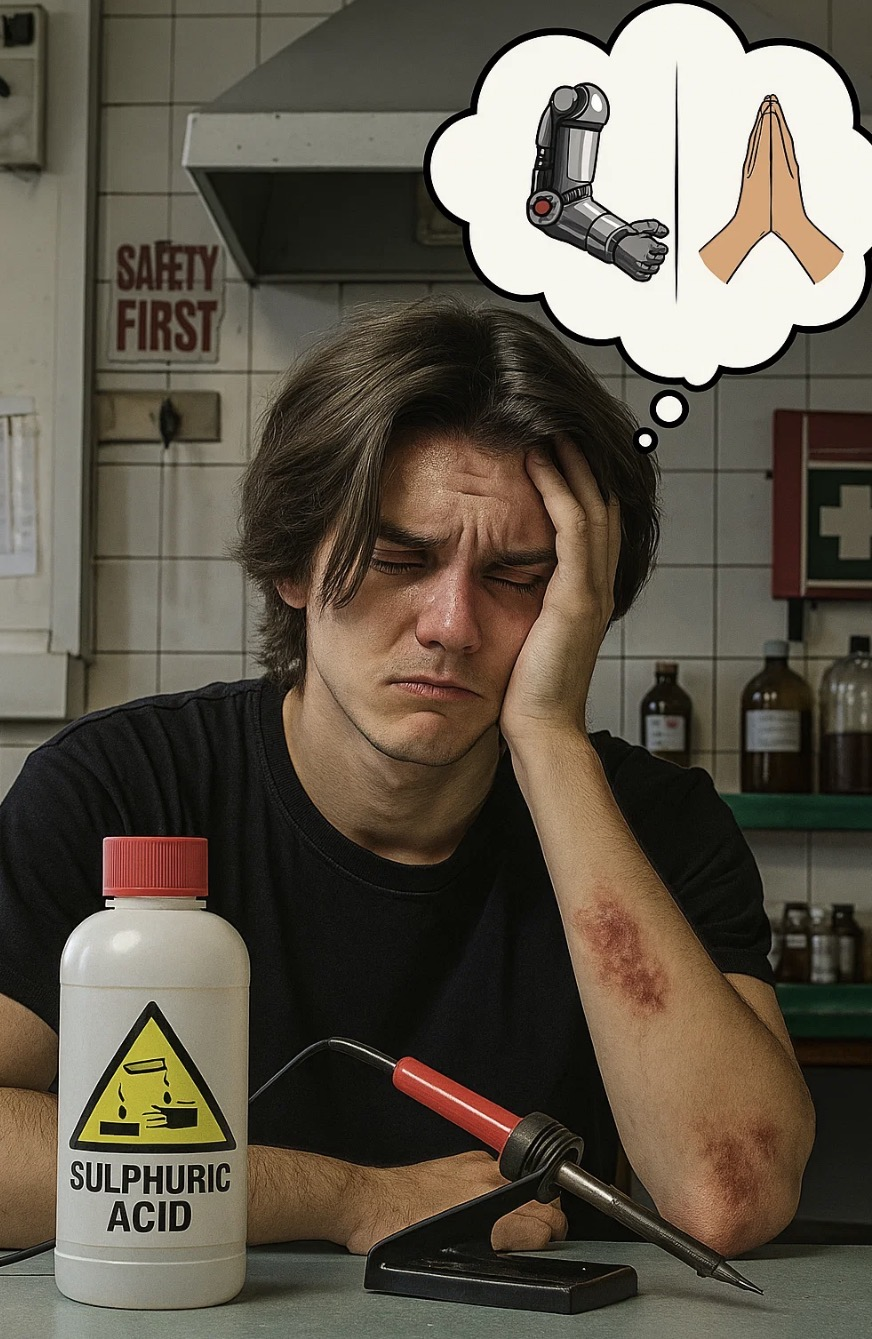
\includegraphics[keepaspectratio, width=.9\textwidth]{david.jpg}
\centering
\caption{How generative AI imagines our problem}
\end{figure}
\end{minipage}\hfill
\begin{minipage}{0.65\linewidth}
\vskip-2\baselineskip
\begin{itemize}
\item Industry is dangerous!
\item Alas! --- if only there were something that would enable us to carry out perilous tasks just as we would with our bare hands, yet without touching the dangerous stuff...
\end{itemize}
\end{minipage}
}

\end{frame}

\begin{frame}{OUR IDEA}
\begin{itemize}
\item To build an interface between the human hand and a custom robotic hand through webcams
\end{itemize}
\end{frame}

\begin{frame}{SEGMENTATION OF THE PROJECT}
\begin{minipage}{0.37\textwidth}
\begin{itemize}
\item System $\alpha$
\begin{figure}
\centering

\includegraphics[keepaspectratio, width=.9\textwidth]
{1.png}
\end{figure}
\end{itemize}
\end{minipage}\hfill
\begin{minipage}{0.62\textwidth}
\begin{itemize}
\item System $\omega$
\begin{figure}
\centering
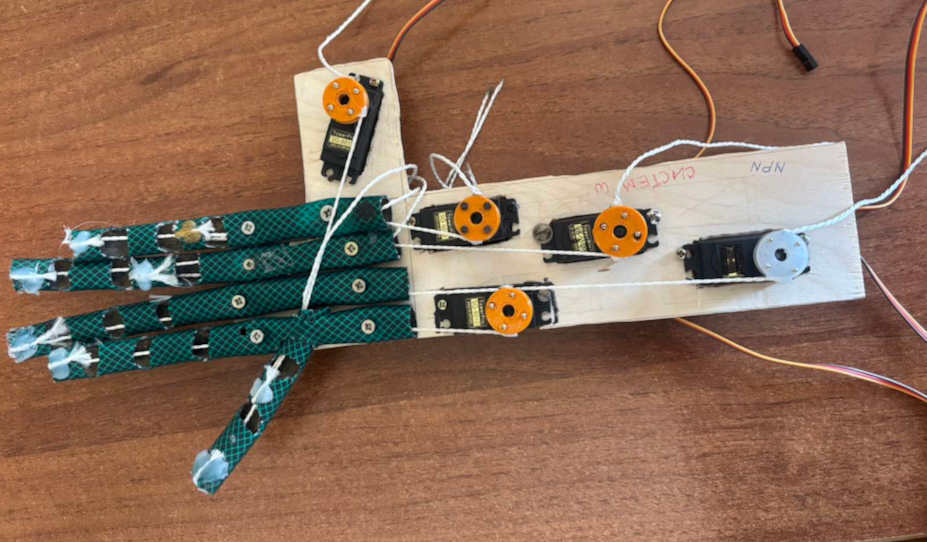
\includegraphics[keepaspectratio, width=.9\textwidth]
{2.png}
\end{figure}
\end{itemize}
\end{minipage}
\end{frame}

\begin{frame}{SYSTEM $\bm{\alpha}$}
\begin{itemize}
\item The image processing segment
\item Comprises a Thinkpad and two webcams on a special stand
\item The webcams have matching $y$ axes and orthogonal $x$ axes, enabling production of images suitable for finger triangulation
\item Tasks it takes care of:
\begin{enumerate}
\item camera calibration
\item image segmentation (finger detection)
\item finger triangulation
\item control number inference
\item message encoding and transmission
\end{enumerate}
\item A special mathematical model of finger movement was conceived so as to satisfy the needs of System $\alpha$ --- the 'Kinderica' Model
\end{itemize}
\end{frame}

\begin{frame}{SYSTEM $\bm{\omega}$}
\begin{itemize}
\item The actuator segment
\item Consists of the robotic hand model, servo motors and an Arduino Uno
\item The hand is fashioned from plywood, garden hose pieces and thin synthetic rope
\item The design leverages the elasticity of rubber
\item Finger movement regulation is achieved through servo motors
\end{itemize}
\end{frame}

\begin{frame}{RESULTS}
\begin{itemize}
\item A functional hand model
\item Successful implementation of numerical control
\item Successful setup of the interface between the subsystems
\item Successful finger triangulation (by colour)
\end{itemize}
\vfill
TO DO (tasks of critical priority):
\begin{itemize}
\item Control number inference
\item Implementation of the 'Kinderica' Model
\item Implementation of ML techniques so as to phase out segmentation by colour
\end{itemize}
\end{frame}

\end{document}
